\documentclass[11pt,a4paper,DIV=14]{scrartcl}
\usepackage[utf8]{inputenc}
\usepackage{fouriernc}
\usepackage[T1]{fontenc}
\usepackage[english]{babel}
\usepackage[hidelinks]{hyperref}
\usepackage{natbib}
\usepackage{url}
\usepackage{amsmath}
\usepackage{amsfonts}
\usepackage{amssymb}
\usepackage{trfsigns}
\usepackage{nicefrac}
\usepackage{graphicx}
\usepackage{caption}
\usepackage{subcaption}
\usepackage{xcolor}
\usepackage{comment}
\usepackage{mdframed}
\usepackage{tikz}
\usepackage{verbatim}

%\usepackage{chngcntr}
%\counterwithout{figure}{subsection}
%\counterwithout{table}{subsection}

\numberwithin{equation}{subsection}
\numberwithin{figure}{subsection}


\bibliographystyle{dinat}

\newcommand\fsd{\mathrm{d}} %Ableitungsoperator
\renewcommand{\vec}[1]{\mathbf{#1}} %Vektor
\newcommand{\eq}[1]{Eq. (\ref{#1})}
\newcommand{\fig}[1]{Fig. \ref{#1}} %Zitat Abbildung
\newcommand{\red}{\textcolor{red}}
\newcommand{\fscom}[2][red]{\textcolor{#1}{#2}}

\usetikzlibrary{shapes.misc}
\tikzset{cross/.style={cross out, draw,
         minimum size=2*(#1-\pgflinewidth),
         inner sep=0pt, outer sep=0pt}}

\definecolor{CalcColor}{rgb}{0.0,0.0,0.5}
\newcommand{\ExCalcCol}[2][CalcColor]{\textcolor{#1}{#2}}
%\excludecomment{calc}
\includecomment{calc}

%##############################################################################
\title{Signal- und Systemtheorie\\
Übung\thanks{
This tutorial is provided as Open Educational Resource (OER), to be found at
\url{https://github.com/spatialaudio/signals-and-systems-exercises}
accompanying the OER lecture
\url{https://github.com/spatialaudio/signals-and-systems-lecture}.
%
Both are licensed under a) the Creative Commons Attribution 4.0 International
License for text and graphics and b) the MIT License for source code.
%
Please attribute material from the tutorial as \textit{Frank Schultz,
Continuous- and Discrete-Time Signals and Systems - A Tutorial Featuring
Computational Examples, University of Rostock} with
\texttt{main file, github URL, commit number and/or version tag, year}.
}
\\
\small Universität Rostock Vst.-Nr. 24015}
%
\author{Dr. Frank Schultz, Prof. Sascha Spors\\
\small Institut für Nachrichtentechnik (INT)\\
\small Fakultät für Informatik und Elektrotechnik (IEF)\\
\small Universität Rostock
}
%
\date{Sommersemester 2020, Version: \today}

%##############################################################################
\begin{document}
\setcounter{section}{2}  % UE 3 in our current sequence
\maketitle
\tableofcontents
\clearpage
\section{UE 3: Solving 2nd Order, Linear, Ordinary Differential Equation with
Constant Coefficients}
\subsection{Problem Statement}
\subsubsection{Electric RLC Circuit}
For a voltage source $u_Q(t)=x(t)$---system input in Volt---connected to a
series circuit consisting of
a resistor with resistance $R$,
an inductor with inductance $L$ and
a capacitor with capacitance $C$,
Kirchhoff's voltage law yields
\begin{align}
\label{eq:KirchhoffLaw}
u_Q(t) = u_R(t) + u_L(t) + u_C(t),
\end{align}
for the system output $y(t) = u_C(t)$ in Volt according to Fig. \ref{fig:lowpass}.
This constitutes a linear and time-invariant (LTI) system describable by impulse
response $h(t)$ and step response $h_\epsilon(t)$.
%
\begin{figure}[h]
\centering
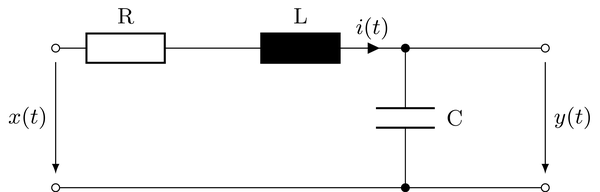
\includegraphics[width=0.5\textwidth]{lowpass.png}
\caption{Electric RLC circuit with current $i(t)$, input voltage $x(t)$
and output voltage $y(t)$.}
\label{fig:lowpass}
\end{figure}



%##############################################################################
\subsubsection{Ordinary Differential Equation (ODE)}
There is one current $i(t)$ flowing in the RLC circuit under discussion.
The corresponding current-voltage laws for the components are
$u_R(t) = R\,i(t)$,
$u_L = L\,\frac{\mathrm{d}i(t)}{\mathrm{d} t}$ and
$u_C(t) = \frac{1}{C} \, \int i(t) \mathrm{d}t$.
With these \eq{eq:KirchhoffLaw} is rewritten as
%
\begin{align}
L C \cdot \ddot{u}_C(t) + R C \cdot \dot{u}_C(t) + u_C(t) = u_Q(t)
\end{align}
using
$\ddot{u}_C(t) = \frac{\mathrm{d}^2 u_C(t)}{\mathrm{d}t^2}$ and
$\dot{u}_C(t) = \frac{\mathrm{d} u_C(t)}{\mathrm{d}t}$
as temporal derivative notations.
%
With
the system input $x(t)$ and
the system output $y(t)$ this 2nd order, linear ODE with
constant coefficients is rewritten
\begin{align}
\label{eq:ODE_RLC}
L C \cdot \ddot{y}(t) + R C \cdot \dot{y}(t) + y(t) = x(t).
\end{align}



%##############################################################################
\subsubsection{Task}
The ODE in \eq{eq:ODE_RLC} with
$R = 3\,\nicefrac{\text{V}}{\text{A}}$,
$L=2\,\nicefrac{\text{V s}}{\text{A}}$,
$C=\frac{8}{25}\,\nicefrac{\text{A s}}{\text{V}}$
is to be solved for $t\geq 0$
\begin{itemize}
\item[a)] $y_\text{particular}(t)$ when $x(t)=\delta(t)$
\item[b)] $y(t) = y_\text{null}(t)+y_\text{particular}(t)$ when
$x(t)=1$ and initial conditions $\dot{y}(0) = 0$, $y(0)=0$
\item[c)] $y(t) = y_\text{null}(t)+y_\text{particular}(t)$ when $x(t)=0$
and initial conditions $\dot{y}(0) = 2$, $y(0)=1$
\item[d)] $y(t) = y_\text{null}(t)+y_\text{particular}(t)$ when $x(t)=1$
and initial conditions $\dot{y}(0) = 2$, $y(0)=1$
\item[e)] $y(t) = y_\text{null}(t)+y_\text{particular}(t)$ when $x(t)=\sin(t)$
and initial conditions $\dot{y}(0) = 0$, $y(0)=0$
\end{itemize}
denoting the Dirac-Delta impulse $\delta(t)$.
%and Heaviside step function
%$\epsilon(t)= \{0\,\,\text{for}\,\,t < 0;\,\,\, 1\,\,\text{for}\,\,t \geq 0\}$.
%
The task shall be performed in the time domain and with the help of the Laplace
transform.
%
Initial conditions refer to the exact time instance $t=0$, excitation signals start
at right limit $t=0+$.



%##############################################################################
%##############################################################################
\subsection{Preliminaries for Fundamental System of Solutions}



%##############################################################################
\subsubsection{Helping Variables}
Before solving any of the requested tasks, it is good scientific and engineering
practice to adapt the ODE for convenient handling and result's interpretation.
Thus (by some experience dealing with such problems and reading text books, cf.
\cite{LangeSigSys1}, \cite{Goeldner1987},  \cite{Oppenheim1997}, \cite{Strang2014}),
we introduce
\begin{equation}
\omega_0^2 = \frac{1}{L C} \rightarrow \omega_0 = \frac{1}{\sqrt{L C}}
\end{equation}
(this is the \textbf{resonance frequency} of the system when no damping would occur)
and
\begin{equation}
\sigma_0 = \frac{1}{2}\frac{R}{L},
\qquad
D = \frac{\sigma_0}{\omega_0}.
\end{equation}
(these are related to the \textbf{damping quality} of the system).
%
Furthermore,
\begin{equation}
\omega_D^2 = \omega_0^2 (1-D^2) \qquad \rightarrow \qquad \omega_D = \omega_0
\sqrt{1-D^2}
\end{equation}
becomes convenient for the case $\sigma_0^2 - \omega_0^2 < 0$.
We will later experience the usefulness of these helping variables.
For now, it is worth to note that $\omega_0$ and $\sigma_0$ intentionally share
\textbf{similarities} with the variable $s=\sigma + \im \omega$ of the
\textbf{Laplace transform}.

By introducing the variables into \eq{eq:ODE_RLC}, we have
\begin{align}
\label{eq:ODE_sigma0}
\boxed{
\frac{\ddot{y}}{\omega_0^2} + \frac{2 \sigma_0}{\omega_0^2} \dot{y} + y = x
}\,,
\end{align}
and
\begin{align}
\label{eq:ODE_D}
\boxed{
\frac{\ddot{y}}{\omega_0^2} + \frac{2 D}{\omega_0} \dot{y} + y = x}\,,
\end{align}
when omitting the temporal dependence $t$ in $y$ and $x$ for brevity.
%
This generalisation allows for discussion of the ODE's characteristics detached
from the underlying physical representation and helps for communication between
engineers with different job specialisation.



%##############################################################################
\subsubsection{Specific Parameters}
With the given values for the electric elements
$R = 3\,\nicefrac{\text{V}}{\text{A}}$,
$L=2\,\nicefrac{\text{V s}}{\text{A}}$,
$C=\frac{8}{25}\,\nicefrac{\text{A s}}{\text{V}}$
we can rewrite \eq{eq:ODE_RLC}
\begin{align}
\boxed{
(\frac{16}{25} \cdot \text{s}^2) \, \ddot{y} + (\frac{24}{25} \cdot \text{s})
\, \dot{y} + y = x.
}
\end{align}
Note that the straight letter s here represents the unit seconds, \textbf{not the Laplace
variable}, which is typeset as italic $s$.
%
The above variables have the quantities
\begin{equation}
\omega_0^2 = \frac{25}{16} \cdot \frac{\text{rad}^2}{\text{s}^2}
\rightarrow \omega_0 = \frac{5}{4} \cdot \frac{\text{rad}}{\text{s}}
\end{equation}
and
\begin{equation}
\sigma_0 = \frac{3}{4}\cdot \frac{\text{1}}{\text{s}}
\qquad D = \frac{3}{5}
\end{equation}
and since $\sigma_0^2 - \omega_0^2 = -1 \cdot \frac{1}{\text{s}^2}< 0\cdot \frac{1}{\text{s}^2}$
\begin{equation}
\omega_D = 1 \cdot \frac{\text{rad}}{\text{s}}.
\end{equation}
%
The chosen values for $R$, $L$, $C$ lead to convenient quantities, which is on
purpose for the upcoming manual calculus. For practical problems we should not
expect such nice numbers.
%
In the remainder we omit the physical units in the calculus.



%##############################################################################
\subsubsection{Homogeneous Solution}
\label{Sec:FundamentalSet}
The present 2nd order ODE can be solved by means of the
fundamental set of solutions
considering the eigenfunctions
\begin{align}
y = \mathrm{e}^{\lambda t}, \quad \lambda\in\mathbb{C}
\end{align}
of the system. Note the (intentional) similarity to $\mathrm{e}^{s t}$,
which is the integral kernel of the Laplace transform.
%
Derivatives with respect to time $t$ become (this is the nice part, why this
works at all)
\begin{align}
y = \mathrm{e}^{\lambda t},\quad
\dot{y} = \lambda \cdot \mathrm{e}^{\lambda t},\quad
\ddot{y} = \lambda^2 \cdot \mathrm{e}^{\lambda t}.
\end{align}
%
We insert these in \eq{eq:ODE_sigma0} with $x=0$, to obtain the
so called \textbf{null solution} $y_\text{null}$, also known as
\textbf{homogeneous solution} $y_h$.
Thus,
\begin{align}
\frac{1}{\omega_0^2} (\lambda^2 \cdot \mathrm{e}^{\lambda t}) +
\frac{2 \sigma_0}{\omega_0^2} (\lambda \cdot \mathrm{e}^{\lambda t}) +
\mathrm{e}^{\lambda t} = 0,\nonumber\\
\label{eq:CharEq}
(\underbrace{\frac{\lambda^2}{\omega_0^2} +
\frac{2 \sigma_0 \lambda}{\omega_0^2} + 1}_\text{characteristic equation})
\cdot \mathrm{e}^{\lambda t} = 0.
\end{align}
%
We are not able to force the left side of this equation to zero with the $\mathrm{e}^{\lambda t}$
function.
Thus, we calculate the zeros of the term within brackets, which is well known as
\textbf{characteristic equation}.
%
The zeros of this 2nd order polynomial are
\begin{align}
\label{lambda12}
\lambda_{1,2} = -\sigma_0 \pm \sqrt{\sigma_0^2 - \omega_0^2}.
\end{align}
%
The homogeneous solution $y_h$ depends on the characteristics
of the term $\sigma_0^2 - \omega_0^2$.
Three cases need to be considered.

\paragraph{Case I for Homogeneous Solution (Kriechfall, starke Dämpfung if $\sigma_0<0$)}
For
\begin{align}
\sigma_0^2 - \omega_0^2 > 0
\end{align}
the Ansatz reads
\begin{align}
y_h=
A \mathrm{e}^{\lambda_1 t} + B \mathrm{e}^{\lambda_2 t}
=
\mathrm{e}^{-\sigma_0 t} [A \mathrm{e}^{+t\,\sqrt{\sigma_0^2 - \omega_0^2}}
+ B \mathrm{e}^{-t\,\sqrt{\sigma_0^2 - \omega_0^2}}]
\end{align}
with the two constants $A$ and $B$ to be defined by the initial conditions
$\dot{y}(t)$ and $y(t)$ for a given $t$ (very often $t=0$)
of the the complete solution
$y(t) = y_\text{null}(t)+y_\text{particular}(t)$.

\paragraph{Case II for Homogeneous Solution (Aperiodischer Grenzfall)}
For
\begin{align}
\sigma_0^2 - \omega_0^2 = 0
\end{align}
a double zero
\begin{align}
\lambda_{1} = \lambda_{2} = -\sigma_0
\end{align}
results for \eq{lambda12}.
Then the Ansatz reads
\begin{align}
y_h = \mathrm{e}^{-\sigma_0 t} [A t + B].
\end{align}

\paragraph{Case III for Homogeneous Solution (Schwingungsfall,
schwache Dämpfung if $\sigma_0<0$)}
\label{pg:caseIII}
For
\begin{align}
\sigma_0^2 - \omega_0^2 < 0,
\end{align}
the already introduced helping variable
\begin{align}
\omega_D^2 = \omega_0^2 - \sigma_0^2 > 0
\end{align}
rearranges \eq{lambda12} to
\begin{align}
\label{eq:lmb12_caseIII}
\lambda_{1,2} = -\sigma_0 \pm \sqrt{-\omega_D^2}
= -\sigma_0 \pm \mathrm{j}\,\omega_D,
\end{align}
yielding a complex conjugate zero pair.
Then the Ansatz reads (cf. case I)
\begin{align}
\label{eq:Ansatz_caseIIIkomplex}
\boxed{
y_h = A \mathrm{e}^{\lambda_1 t} + B \mathrm{e}^{\lambda_2 t}.
}
\end{align}
or (using other $A$, $B$)
\begin{align}
\label{eq:Ansatz_caseIIIsincos}
y_h = \mathrm{e}^{-\sigma_0 t}
\left[ A \sin(\omega_D t) + B \cos(\omega_D t)\right].
\end{align}
While \eq{eq:Ansatz_caseIIIkomplex} is more elegant to perform calculus,
\eq{eq:Ansatz_caseIIIsincos} directly reveals the \textbf{damped}
(parameter $\sigma_0$) sine and cosine \textbf{oscillations}
(with angular frequency $\omega_D$).
%
Case III covers the characteristics of the majority of practical systems
for signal processing.



%##############################################################################
\subsubsection{Inhomogeneous Solution}
Now, let the ODE be of form
\begin{align}
a \, \ddot{y} + b \, \dot{y} + c \, y = x.
\end{align}
with constant coefficients $a, b, c\in \mathbb{R}$.
%
There are different suitable approaches for solving such an ODE for
different inhomogeneities $x$.
We restrict our discussion to the most often asked cases.
We should check our math lecture notes for e.g. the method
\textit{variation of parameters / Variation der Konstanten} for a general
solution concept, cf. \cite{Burg2013}.

\paragraph{Polynomial Function}
The particular solution $y_p$ for the inhomogeneous ODE with
polynomial $x = P_n(t)$ of degree $n$
(for example $x = p_n t^n + p_{n-1} t^{n-1} + ... +p_0$)
requires the Ansatz
\begin{align}
y_p =
\begin{cases}
Q_n(t)&\quad a\neq 0, c\neq 0\\
t Q_n(t)&\quad a\neq 0, b\neq 0, c=0\\
t^2 Q_n(t)&\quad a\neq 0, b=0, c=0
\end{cases}
\end{align}
and solving for the coefficients $q_n, q_{n-1},...,q_0$ by comparing
coefficients in
\begin{align}
a \, \ddot{y}_p + b \, \dot{y}_p + c \, y_p = x.
\end{align}

\paragraph{Exponential Function (i.e. Eigenfunctions of the ODE)}
The particular solution $y_p$ for the inhomogeneous ODE with
$x = \e^{s_x t}$
requires the Ansatz
\begin{align}
y_p =
\begin{cases}
A \cdot \e^{s_x t}&\quad \text{if} \quad  s_x \notin \lambda_{1,2}\\
A t \cdot \e^{s_x t}&\quad \text{if} \quad s_x \in \lambda_{1 \text{ or } 2}\\
A t^2 \cdot \e^{s_x t}&\quad \text{if} \quad s_x \in \lambda_{1 \text{ and } 2}
\end{cases}
\end{align}
and solving for the coefficient $A$ by comparing coefficients.

\paragraph{Cosine / Sine Functions (i.e. Special Case of ODE's Eigenfunctions)}
\label{Sec:CosSineAnsatzInhomo}
The particular solution $y_p$ for the inhomogeneous ODE with
$x=\sin(\omega_x t)$ or $x=\cos(\omega_x t)$
requires the Ansatz
\begin{align}
y_p =
\begin{cases}
A \cdot \cos(\omega_x t) + B \cdot \sin(\omega_x t)&\quad \text{if}
\quad \im \omega_x \notin \lambda_{1,2}\\
A t \cdot \cos(\omega_x t) + B t \cdot \sin(\omega_x t)&\quad \text{if}
\quad \im \omega_x \in \lambda_{1,2}
\end{cases}
\end{align}
and solving for the coefficients $A, B$ by comparing coefficients.



%##############################################################################
\subsubsection{Full ODE Solution}
The full solution of an ODE is the superposition of the homogeneous solution
and inhomogeneous (particular) solution
\begin{align}
y(t) = y_\text{null}(t)+y_\text{particular}(t) \qquad \rightarrow \qquad
y = y_h + y_p
\end{align}
and then resolving for the initial conditions $\dot{y}(t)$ and $y(t)$ for a
given $t$ (very often $t=0$) to obtain the specific solution $y$.



%##############################################################################
%##############################################################################
\subsection{Solutions Using Fundamental System}



%##############################################################################
\subsubsection{Task a) with Fundamental System / Impulse Response}
We shall solve
\begin{align}
\frac{16}{25} \ddot{y} + \frac{24}{25} \dot{y} + y = \delta(t)
\end{align}
for the particular solution $y_p$ in the time domain.

%
A brilliant didactical approach tailored for engineers to solve this task is
found in \cite{Strang2014}.
%
In short, the \textbf{particular solution} $y_p(t)$ of this equation
with \textbf{Dirac impulse excitation} is named the \textbf{Green's function} $g(t)$.
%
When the null solutions of the ODE are known, the Green's function can be found
by variation of parameters.
Making use of the important sifting property
$\int\limits_{-\infty}^{+\infty} \delta(t-t_0) \cdot f(t) \, \mathrm{d} t \stackrel{\mathrm{def}}= f(t_0)$
becomes a vital part when doing this.
%
However, we will not go into detail here, cf. \cite[p.133]{Strang2014} instead.
%
The important part of the story is:
Once $g(t)$ is known,
the \textbf{particular solution} $y_p$ \textbf{for any other inhomogeneity}
$x(t)$ can be derived with the \textbf{convolution} operation
$y_p(t) = x(t) * g(t)$.
%
This constitutes a fundamental (if not the most important) theorem for ODEs.
%
For our discussed ODEs in signal and
system theory (where we only handle time dependence), we call the Green's
function $g(t)$ typically the \textbf{impulse response} $h(t)$ of the
\textbf{LTI system} and use the convolution $y_p(t) = x(t) * h(t)$.

\textbf{Important detail}: Actually the initial conditions problem
$\frac{16}{25} \ddot{h}(t) + \frac{24}{25} \dot{h}(t) + h(t) = \delta(t), h'(0-)=0, h(0-)=0$
solves for the impulse response, where we need the left sided limit $t=0-$,
since the Dirac impulse excites at $t=0$.
%
This proof is a little bit off-topic due to lack of time.
%
Instead, we can use the particular solution only by keeping in
mind that the system was in rest before excitation.

Said that, we can make our life even more convenient, since according to
\cite[p.97]{Strang2014},
the \textbf{Green's function is also found by the null solution}
(instead of Dirac excitation)
\textbf{and new specific initial conditions}.
In general for a 2nd order ODE this means
%\begin{align}
$a \, \ddot{y} + b \, \dot{y} + c \, y = 0,
\quad y(0)=0,
\quad \dot{y}(0)=\frac{1}{a}$,
%\end{align}
and thus for our specified example
\begin{align}
\frac{16}{25} \ddot{y} + \frac{24}{25} \dot{y} + y = 0,
\quad y(0)=0,
\quad \dot{y}(0)=\frac{25}{16}
\end{align}
for $t\geq 0$.
%
Feel free to explore the solution by usage of \url{https://www.wolframalpha.com}
with the input \verb|16/25*y’’(t)+24/25*y’(t)+y(t)=0, y(0)=0, y'(0)=25/16|
or with other tools that can handle symbolic math on a computer.
%
We are going to calculate this manually in the following.
%


\paragraph{Homogeneous Solution}
\label{Sec:TaskaHomo}
First, we need the homogeneous solution of the ODE for this subtask.
%
We will also need this in general, so it is anyway a good idea to calculate
this first.
%
According to Sec. \ref{Sec:FundamentalSet} the characteristic equation for the
ODE is \eq{lambda12}
\begin{align}
\lambda_{1,2} = -\sigma_0 \pm \sqrt{\sigma_0^2 - \omega_0^2}.
\end{align}
and with the chosen quantities, we get
\begin{align}
\lambda_{1,2} = -\frac{3}{4} \pm \im,
\end{align}
i.e. a complex conjugate zero pair with intentionally very simple numbers.
Thus, we deal with \textbf{case III} (page \pageref{pg:caseIII})
for the homogeneous solution, this is the case of \textbf{damped oscillation}.
The corresponding zero pair is depicted in Fig.~\ref{fig:sketch_lambda_plane},
left.
%
Repeating \eq{eq:lmb12_caseIII}
$\lambda_{1,2} = -\sigma_0 \pm \mathrm{j}\omega_D$,
we identify $\sigma_0 = \frac{3}{4}$ and $\omega_D = 1$.
Repeating \eq{eq:Ansatz_caseIIIkomplex}
$y_h = A \mathrm{e}^{\lambda_1 t} + B \mathrm{e}^{\lambda_2 t}$,
we therefore have to deal with
\begin{align}
y_h = A \, \mathrm{e}^{(-\frac{3}{4}+\im)\,t} + B \, \mathrm{e}^{(-\frac{3}{4}-\im)\,t},
\end{align}
and since $y_p=0$
\begin{align}
y = y_h + y_p = A \, \mathrm{e}^{(-\frac{3}{4}+\im)\,t} + B \, \mathrm{e}^{(-\frac{3}{4}-\im)\,t}.
\end{align}

\paragraph{Initial Conditions}
\label{Sec:TaskaInitCond}
The initial conditions $y(0)=0$ and $\dot{y}(0)=\nicefrac{25}{16}$ require to find
the derivative
\begin{align}
\dot{y} =
(-\frac{3}{4}+\im) A \, \mathrm{e}^{(-\frac{3}{4}+\im)\,t} +
(-\frac{3}{4}-\im) B \, \mathrm{e}^{(-\frac{3}{4}-\im)\,t}.
\end{align}
%
The ease of performing this derivation makes the Ansatz \eq{eq:Ansatz_caseIIIkomplex}
more elegant than \eq{eq:Ansatz_caseIIIsincos}.
%
However, we now have slightly more effort to find the coefficients $A$ and $B$,
but it is actually more enlightening, how our final result evolves.
%
Applying the initial conditions yields
%
\begin{align}
y(0) = 0 = A + B
\qquad
\dot{y}(0) = \nicefrac{25}{16} =
(-\frac{3}{4}+\im) \, A + (-\frac{3}{4}-\im) \, B
\end{align}
Thus, comparing coefficients and using one Euler identity
$\sin(x) = \frac{\e^{\im x}-\e^{-\im x}}{2\im}$
\begin{align}
A = \frac{\nicefrac{25}{16}}{2\im}\qquad B = -\frac{\nicefrac{25}{16}}{2\im}
\quad\rightarrow\quad
y = y_h + y_p =
 \frac{\nicefrac{25}{16}}{2\im} \, \mathrm{e}^{(-\frac{3}{4}+\im)\,t}
-\frac{\nicefrac{25}{16}}{2\im} \, \mathrm{e}^{(-\frac{3}{4}-\im)\,t},
\end{align}
yields the \textbf{impulse response} of the 2nd order system / ODE under discussion
\begin{align}
\boxed{
h = y_\text{Task a} = \nicefrac{25}{16} \cdot \mathrm{e}^{-\frac{3}{4} t} \sin(t) \qquad t\geq0
}\,.
\end{align}



%##############################################################################
\subsubsection{Task b) with Fundamental System / Step Response}
We shall solve
\begin{align}
\frac{16}{25} \ddot{y} + \frac{24}{25} \dot{y} + y = 1, \quad
\dot{y}(0) = 0,\quad y(0)=0
\end{align}
for $y$ with the Ansatz of fundamental set of solutions.

\paragraph{Inhomogeneous Solution}
The source term $x(t\geq 0+)=1$ exhibits unit
amplitude over time. This can be stated as the most simple polynomial $p_0=1$.
Thus, the polynomial Ansatz $y_p = q_0$ leads to
\begin{align}
\frac{16}{25} \ddot{y}_p + \frac{24}{25} \dot{y}_p + y_p = 1
\rightarrow q_0 = 1 \rightarrow  y_p = 1.
\end{align}

\paragraph{Specific Solution with Initial Conditions}
The superposition of the homogeneous (this timewe use the sin/cos-Ansatz
\eq{eq:Ansatz_caseIIIsincos} for demonstration purpose) and the inhomogeneous
solution is
\begin{align}
\label{eq:SpecificyTaskb}
y = y_h + y_p = \underbrace{
\mathrm{e}^{-\frac{3}{4} t} \cdot
\left[ A \sin(t) + B  \cos(t)\right]}_{y_h} +\underbrace{1}_{y_p}.
\end{align}
The initial condition $\dot{y}(0) = 0$ again requires to find the derivative
\begin{align}
\dot{y}
=
-\frac{3}{4}\mathrm{e}^{-\frac{3}{4} t} \cdot
\left[ A \sin(t) + B \cos(t)\right]
+
\mathrm{e}^{-\frac{3}{4} t} \cdot
\left[ A \cos(t)  - B \sin(t)\right].
\end{align}
The initial condition $\dot{y}(0) = 0$ yields
\begin{align}
0 = -\frac{3}{4}\cdot B + A \rightarrow A = \frac{3}{4}\cdot B.
\end{align}
The initial condition ${y}(0) = 0$ yields
\begin{align}
0 = B  + 1 \rightarrow B = -1.
\end{align}
The resulting coefficients
\begin{align}
A = -\frac{3}{4}\qquad B = -1
\end{align}
are inserted into \eq{eq:SpecificyTaskb}
\begin{align}
\boxed{
h_\epsilon = y_\text{Task b} =
1 - \mathrm{e}^{-\frac{3}{4} t} \cdot
\left(\frac{3}{4} \sin(t) + \cos(t)\right) \qquad t \geq 0
}\,,
\end{align}
giving the final result for task b) with $h_\epsilon(t\to\infty) = 1$.

In Fig.~\ref{fig:step_response_parts} the solution $y_\text{Task b}$ is depicted
as the thick, non-dashed orange graph. It results from the superposition of the
functions
i. unit amplitude (black),
ii. exponentially damped, negative sine (green, diamonds),
iii. exponentially damped, negative cosine (red, stars).
In grey colour, the pure sine and cosine functions with negative amplitude,
as well as the exponential
damping with different initial amplitude are indicated.

\begin{figure}[h!]
\centering
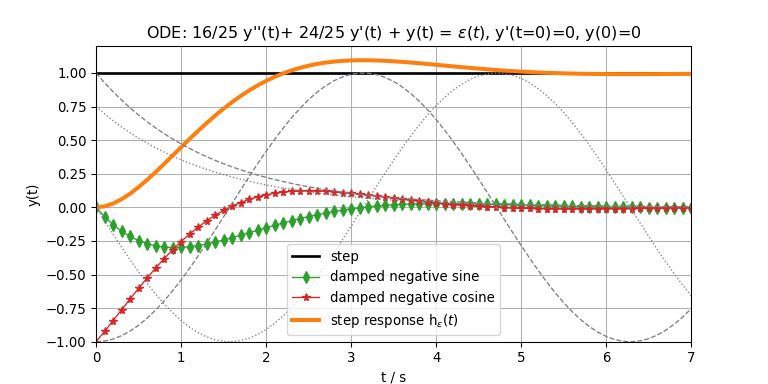
\includegraphics[width=0.75\textwidth]{step_response_parts}
\caption{Response of task b for ODE under discussion.}
\label{fig:step_response_parts}
\end{figure}

Feel free to double check this solution at Wolfram Alpha with input
\begin{verbatim}
16/25*y''(t)+24/25*y'(t)+y(t)=1,       y'(0)=0, y(0)=0
16/25*y''(t)+24/25*y'(t)+y(t)=Step[t], y'(0)=0, y(0)=0
\end{verbatim}




%##############################################################################
\subsubsection{Task a) Revisited with Fundamental System / Impulse Response}
%
The Heaviside step function
\begin{equation}
\epsilon(t) =
\begin{cases}
  0 & t\leq 0-\\
  1 & t\geq 0+
\end{cases}
\end{equation}
and
the Dirac impulse $\delta(t)$ are related by
\begin{align}
\dot{\epsilon}(t) = \delta(t).
\end{align}
In fact, in task a and b we just derived the impulse response $h$ and step response
$h_\epsilon$ of the ODE, respectively.
%
We can also relate the step and impulse response by
\begin{align}
\dot{h_\epsilon}(t) = h(t).
\end{align}
%
The \textbf{temporal derivative of the step response} $h_\epsilon=y_\text{Task b}$
\textbf{yields the impulse response} $h$.
Thus, for the step response
\begin{align}
h_\epsilon = y_\text{Task b} =
1 - \mathrm{e}^{-\frac{3}{4} t} \cdot
\left( \frac{3}{4} \sin(t) + \cos(t)\right)
\end{align}
the derivative is the impulse response
\begin{align}
h = \dot{h_\epsilon} = \dot{y}_\text{Task b} =
 - (-\frac{3}{4})\,\mathrm{e}^{-\frac{3}{4} t} \cdot
\left( \frac{3}{4} \sin(t) + \cos(t)\right)
- \mathrm{e}^{-\frac{3}{4} t} \cdot
\left( \frac{3}{4} \cos(t) - \sin(t)\right).
\end{align}
Rearranging yields the expected result identical to task a
\begin{align}
\boxed{
h = y_\text{Task a} = \frac{25}{16} \mathrm{e}^{-\frac{3}{4} t} \sin(t) \qquad t\geq 0
}\,.
\end{align}
%
In Fig. \ref{fig:impulse_step_response} the impulse response is depicted as
the dashed blue graph, whereas the step response is plotted in thick
orange again.
The impulse response is a weighted and exponentially damped sine function
with $h(t\to\infty) = 0$.

\begin{figure}[h!]
\centering
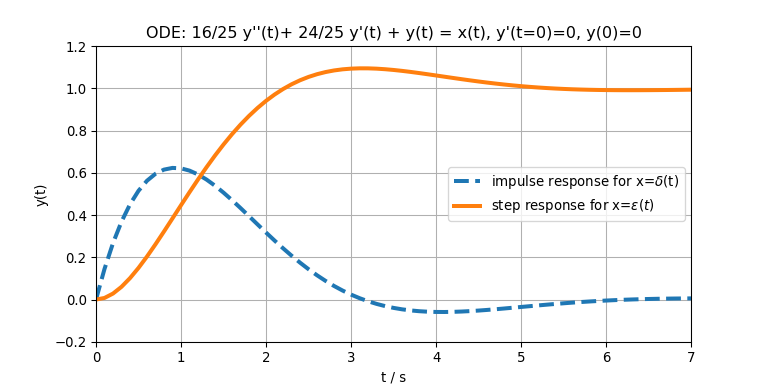
\includegraphics[width=0.75\textwidth]{impulse_step_response}
\caption{Impulse response (task a, blue, dotted) and step response (task b, orange, thick)
of the ODE under discussion.}
\label{fig:impulse_step_response}
\end{figure}

Feel free to verify that Wolfram Alpha returns the particular solution to the
input
\begin{verbatim}
16/25*y''(t)+24/25*y'(t)+y(t)=DiracDelta[t]
\end{verbatim}
precisely identical to the manually calculated impulse response.



%##############################################################################
\subsubsection{Task c) with Fundamental System}
Now, we shall solve
\begin{align}
\frac{16}{25} \ddot{y} + \frac{24}{25} \dot{y} + y = 0,
\quad \dot{y}(0) = 2,\quad y(0)=1
\end{align}
for $y$.
%
Since $y_p=0$, we can immediately adapt the solution of Sec.
\ref{Sec:TaskaHomo} and \ref{Sec:TaskaInitCond} as
%
\begin{align}
y_h + y_p = y =& A \, \mathrm{e}^{(-\frac{3}{4}+\im)\,t} + B \, \mathrm{e}^{(-\frac{3}{4}-\im)\,t}\\
\dot{y} =&
(-\frac{3}{4}+\im) A \, \mathrm{e}^{(-\frac{3}{4}+\im)\,t} +
(-\frac{3}{4}-\im) B \, \mathrm{e}^{(-\frac{3}{4}-\im)\,t}
\end{align}
%
Applying the initial conditions yields
%
\begin{align}
\dot{y}(0) = 2 =
(-\frac{3}{4}+\im) A+
(-\frac{3}{4}-\im) B
\qquad
y(0) = 1 = A + B.
\end{align}
Thus, the coefficients become
\begin{align}
A = \frac{1}{2} + \frac{11}{8\im}\qquad B = 1-A = \frac{1}{2} - \frac{11}{8\im}.
\end{align}
%
Inserting these and applying the Euler identities
$\cos(x) = \frac{\e^{\im x}+\e^{-\im x}}{2}$,
$\sin(x) = \frac{\e^{\im x}-\e^{-\im x}}{2\im}$
yields
\begin{align}
\boxed{
y_\text{Task c} = \mathrm{e}^{-\frac{3}{4} t} \cdot
\left( \frac{11}{4} \sin(t) + \cos(t)\right) \qquad t\geq 0
}\,.
\end{align}
In Fig.~\ref{fig:initial_conditions_response_parts} the brown graph depicts the
response $y_\text{Task c}$, which is decaying to zero since the L and C are
just discharging. As typical for such ODEs, again
weighted and exponentially damped cosine (red, stars) and sine (green, diamonds)
function are superimposed.

\begin{figure}[h!]
\centering
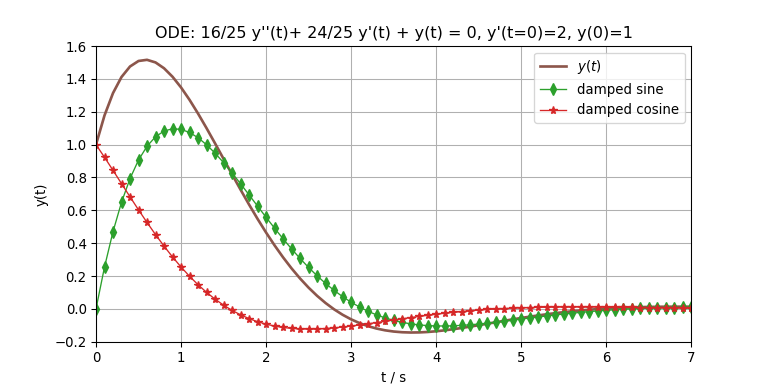
\includegraphics[width=0.75\textwidth]{initial_conditions_response_parts}
\caption{Response of task c for the ODE with initial conditions but no external input.}
\label{fig:initial_conditions_response_parts}
\end{figure}

Feel free to double check this solution at Wolfram Alpha with input
\begin{verbatim}
16/25*y''(t)+24/25*y'(t)+y(t)=0, y'(0)=2, y(0)=1
\end{verbatim}



%##############################################################################
\subsubsection{Task d) with Fundamental System}
In this task we shall solve
\begin{align}
\frac{16}{25} \ddot{y} + \frac{24}{25} \dot{y} + y = 1, \quad
\dot{y}(0) = 2,\quad y(0)=1
\end{align}
for $y$.
%
This task is the \textbf{superposition} of the solution from \textbf{task b} (exterior source
but vanishing initial conditions) and the solution of \textbf{task c} (no exterior
source, but initial conditions). Thus, we should expect
\begin{align}
&y_\text{Task d} =
y_\text{Task b} +
y_\text{Task c} = 1 + 2\mathrm{e}^{-\frac{3}{4} t} \sin(t) = \nonumber\\
&\left[1 - \mathrm{e}^{-\frac{3}{4} t} \cdot
\left( \frac{3}{4} \sin(t) + \cos(t)\right)\right]
+\left[\mathrm{e}^{-\frac{3}{4} t} \cdot
\left( \frac{11}{4} \sin(t) + \cos(t)\right)\right].
\end{align}
%
In order to reassure this result, we can start with \eq{eq:SpecificyTaskb} from
task b and rearrange this for the differing initial conditions:
The superposition of the homogeneous and inhomogeneous solution is
\begin{align}
y = y_h + y_p = \underbrace{
\mathrm{e}^{-\frac{3}{4} t} \cdot
\left( A \sin(t) + B \cos(t)\right)}_{y_h} + \underbrace{1}_{y_p}
\end{align}
Again, derivation with respect to time is
\begin{align}
\dot{y}
=
-\frac{3}{4}\,\mathrm{e}^{-\frac{3}{4} t} \cdot
\left( A \sin(t) + B \cos(t)\right)
+
\mathrm{e}^{-\frac{3}{4} t} \cdot
\left( A \cos(t)  - B \sin(t)\right).
\end{align}
The initial condition $\dot{y}(0) = 2$ yields
\begin{align}
2 = -\frac{3}{4}\cdot B + A \rightarrow A = 2 +  \frac{3}{4}\cdot B.
\end{align}
The initial condition ${y}(0) = 1$ yields
\begin{align}
1 = B  + 1 \rightarrow B = 0.
\end{align}
Thus,
\begin{align}
A = 2\qquad B = 0
\end{align}
inserted
\begin{align}
\boxed{
y_\text{Task d} =
1+\mathrm{e}^{-\frac{3}{4} t}
\, 2 \sin(t)\qquad t \geq 0
}
\end{align}
leads to the final result for task d) as expected.
%
\begin{figure}[b!]
\centering
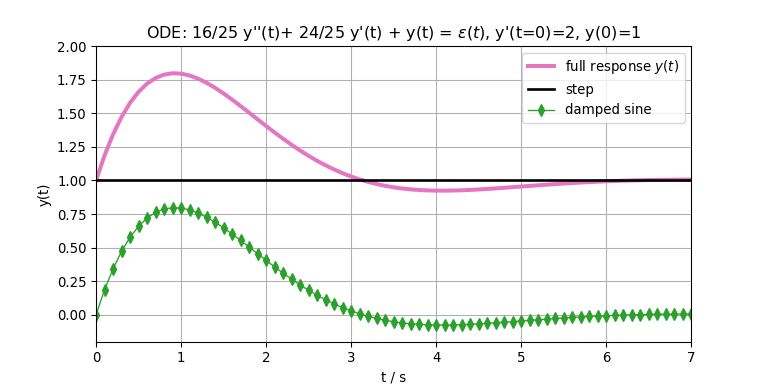
\includegraphics[width=0.75\textwidth]{response_full}
\caption{Response of task d for the ODE with initial conditions and step input.}
\label{fig:response_full}
\end{figure}
%
In Fig.~\ref{fig:response_full} the response $y_\text{Task d} $ is depicted as
magenta graph. This is the result of the superposition of the Heaviside step
function and an exponentially damped, weighted sine function.
The final result asymptotically converges to unit amplitude.
%
This is expected: once the initial conditions are vanished for $t\to\infty$
the external excitation of the step function is the dominant part for the system
response.
%
We can see this in the equations: $y_\text{Task d}(t\to\infty) = y_\text{Task b}(t\to\infty)$

Feel free to double check this solution at Wolfram Alpha with input
\begin{verbatim}
16/25*y''(t)+24/25*y'(t)+y(t)=1, y'(0)=2, y(0)=1
\end{verbatim}





%##############################################################################
\subsubsection{Task e) with Fundamental System}
In this task we shall solve
\begin{align}
\label{eq:InHomoODE_sin}
\frac{16}{25} \ddot{y} + \frac{24}{25} \dot{y} + y = \sin(t), \quad
\dot{y}(0) = 0,\quad y(0)=0
\end{align}
for $y$.
%
We already know the homogeneous solution
$y_h = \mathrm{e}^{-\frac{3}{4} t} \cdot
\left[ A \sin(t) + B \cos(t)\right]$.
%
The inhomogeneity in this case can be solved with the Ansatz (cf.
Sec. \ref{Sec:CosSineAnsatzInhomo})
\begin{align}
y_p = C \sin(t) + D \cos(t).
\end{align}
Inserting this into \eq{eq:InHomoODE_sin}, the
coefficients are solved to
\begin{align}
C = \frac{25}{73}\qquad D = -\frac{200}{219}.
\end{align}
%
The solution then becomes
\begin{align}
y = y_h + y_p = \underbrace{\mathrm{e}^{-\frac{3}{4} t} \cdot
\left[ A \sin(t) + B \cos(t)\right]}_{\text{damped solution} \, y_h}+
\underbrace{\frac{25}{73} \sin(t) - \frac{200}{219} \cos(t)}_{\text{oscillating solution} \, y_p}.
\end{align}
By considering the initial conditions the remaining unknown coefficients solve to
\begin{align}
A = \frac{25}{73}\qquad B = \frac{200}{219}
\end{align}
giving the final result
\begin{align}
\boxed{
y_\text{Task e} = \frac{25}{73} \mathrm{e}^{-\frac{3}{4} t} \sin(t) +
\frac{200}{219} \mathrm{e}^{-\frac{3}{4} t} \cos(t) +
\frac{25}{73} \sin(t) -
\frac{200}{219} \cos(t) \qquad t\geq 0
}\, ,
\end{align}
%
\begin{figure}[h!]
\centering
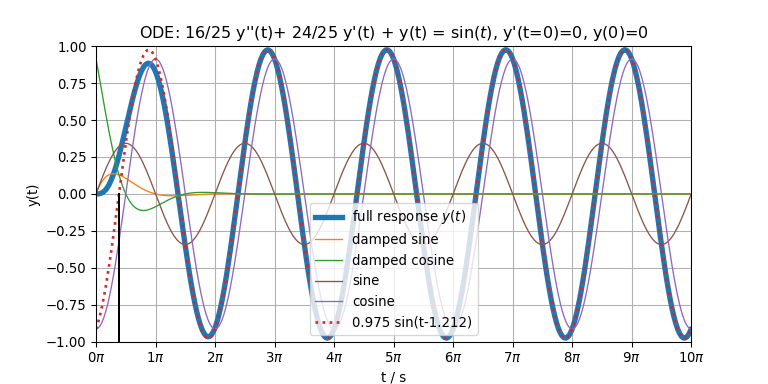
\includegraphics[width=0.75\textwidth]{sine_excitation_response}
\caption{Response of task e for the ODE with zero initial conditions and
$\sin(t)$ input.}
\label{fig:sine_excitation_response}
\end{figure}

The response is depicted in Fig.~\ref{fig:sine_excitation_response} in
thick/blue.
It results from the superposition of i. weighted and \textbf{exponentially damped}
sine and cosine functions (yellow and green graphs) and ii. weighted but \textbf{undamped}
sine and cosine functions (brown and purple graphs).

\subsubsection{Steady State of the System}
%
In this example it is important to realise that the initial conditions
(exponentially damped sine and cosine) contribute
to the system response only up to approximately $t=2\pi$
seconds, i.e. in the first period $T=\frac{2\pi}{\omega_D}=2\pi$ of the
excitation's frequency here.
%
For times $t\gg2\pi$ seconds the system response is determined by the
undamped sine and cosine functions, yielding a system response of
\begin{align}
\label{eq:steadystate_timedomain}
y(t\gg 2\pi, t\to\infty) = \frac{25}{3 \sqrt{73}}\cdot
\sin\left(t-\tan^{-1}
\left[\frac{\nicefrac{200}{219}}{\nicefrac{25}{73}}\right]\right),
\end{align}
depicted as the red dotted graph in Fig.~\ref{fig:sine_excitation_response}.
This constitutes the so called \textbf{steady-state} of the system response
for $t\to\infty$.
For that, we see that the excitation signal $x=\sin(t)$ is altered in amplitude
(very subtle damping of about 0.975) and
a time delay (in terms of phase: about -70 degrees or about $-0.386 \pi$ in
radian), cf. the black line indicator in the figure.
Note that $\frac{\nicefrac{200}{219}}{\nicefrac{25}{73}} = \nicefrac{8}{3}$ again
results in simple numbers for the chosen example. We will rather not see such
for real practical problems.

The two parameters in the
\textbf{steady state}---\textbf{the amplitude and the phase offset}---and
their specific quantities are very important for the
interpretation of ODEs as LTI systems. Each excitation frequency has its own
quantity set, yielding frequency dependent system characteristics.
We will deal with it in detail when discussing ODEs in Laplace domain.
%
The so called Bode plot or \textbf{Bode diagram} is one still important tool
to visualize amplitude and phase over frequency in approximated manner.

Feel free to double check this solution at Wolfram Alpha with input
\begin{verbatim}
16/25*y''(t)+24/25*y'(t)+y(t)=Sin[t], y'(0)=0, y(0)=0
\end{verbatim}





%##############################################################################
\subsection{Preliminaries for Laplace Transform}
We should now study the problem with the help of the Laplace transform.
For the chosen ODE and input signals the calculus effort is about the same,
however for more complicated cases, the approach via Laplace transform
is often the more convenient approach for the solution.
%
For instance, Laplace transform is more powerful, when the \textbf{steady state}
system response for oscillations \textbf{at many different frequencies} is
searched for.
%
Instead of solving each individual problem with the approach that we took before,
the problem is conveniently solved by means of the \textbf{transfer function},
which stores amplitude and phase offset for each arbitrary oscillation frequency.
%
We will discover this, when solving tasks a) to e) with the help of the Laplace
transform. The solutions must be of course identical to these we have found so far.

To obtain the time function the inverse Laplace function is needed.
%
We do not need to use the complex integral and application of the
\textbf{residue theorem}
here, but rather make use of \textbf{correspondence tables for Laplace transforms}.
%
The English and German textbooks
\cite{Strang2014,GirodRabensteinStenger2007,Girod2001,Oppenheim1997,Fliege1991,
Goeldner1987,LangeSigSys1,Wunsch1972}
can be considered classics and cover the Laplace transform very well for our
purpose.




%##############################################################################
\subsubsection{Laplace Transform Fundamentals}
The Laplace transform pair reads
\begin{align}
Y(s) = \mathcal{L}\{y(t)\}= \int\limits_{-\infty}^{\infty} y(t) \e^{-s t}
\mathrm{d} t\qquad
y(t) = \mathcal{L}^{-1}\{Y(s)\}= \frac{1}{2\pi\im}\int
\limits_{\sigma-\im \infty}^{\sigma+\im\infty} Y(s) \e^{+s t} \mathrm{d} s.
\end{align}
We use the operators
$y(t) \quad \laplace \quad Y(s)$ and
$Y(s) = \mathcal{L}\{y(t)\}$
to indicate forward Laplace transform.
We use the operators
$Y(s) \quad \Laplace \quad y(t)$ and
$y(t) = \mathcal{L}^{-1}\{Y(s)\}$
to indicate inverse Laplace transform.

To make the Laplace transform helpful for solving ODEs, we first reconsider
that the Laplace transform is linear, i.e. it preserves scaling and
superposition in both signal domains
\begin{align}
A y_1(t) + B y_2(t) \quad \laplace \quad A Y_1(s) + B Y_2(s).
\end{align}
The second, fundamental important characteristics of the Laplace transform is
\begin{align}
\mathcal{L}\{\frac{\mathrm{d}^n y(t)}{\mathrm{d} t^n}\}=
s^n Y(s) - \sum_{k=1}^{n} s^{n-k} \cdot
\frac{\mathrm{d}^{k-1} y(t)}{\mathrm{d} t^{k-1}}\bigg|_{t=0},
\end{align}
The temporal derivation operation will be transformed to a multiplication
operation with Laplace variable $s$ (\textbf{differential equations} essentially \textbf{become
algebraic equations}, that is the key idea and a special case of
so called operator theory, we have seen a similar concept already for the
characteristic polynomial).
%
For typical systems up to 2nd order, we will need
\begin{align}
\label{eq:Laplace0thd}
\boxed{\mathcal{L}\{{y(t)}\} = Y(s)},
\end{align}
\begin{align}
\label{eq:Laplace1std}
\mathcal{L}\{\frac{\mathrm{d} y(t)}{\mathrm{d} t}\}=
s \cdot Y(s) - \sum_{k=1}^{1} s^{1-k} \cdot
\frac{\mathrm{d}^{k-1} y(t)}{\mathrm{d} t^{k-1}}\bigg|_{t=0}
= \boxed{\mathcal{L}\{\dot{y}\} = s \cdot Y(s) - y(0)}
\end{align}
and
\begin{align}
\label{eq:Laplace2ndd}
\mathcal{L}\{\frac{\mathrm{d}^2 y(t)}{\mathrm{d} t^2}\}=
s^2 \cdot Y(s) - \sum_{k=1}^{2} s^{2-k} \cdot
\frac{\mathrm{d}^{k-1} y(t)}{\mathrm{d} t^{k-1}}\bigg|_{t=0}
= \boxed{\mathcal{L}\{\ddot{y}\} = s^2 \cdot Y(s) - s \cdot y(0) - \dot{y}(0)}\,.
\end{align}

Note the \textbf{application of the initial conditions} in these transform rules!

%##############################################################################
\subsubsection{Algorithm for Solving ODEs via Laplace Transform}

Solving an ODE problem via the indirect way of Laplace transform is then as follows
\begin{itemize}
\item[1.] transform the ODE equation to the Laplace domain by applying linearity and
derivative rules
\item[2.] insert the initial conditions of $y(0)$  and $\dot{y}(0)$
(if they are zero, actually the additional terms immediately become zero,
this is very nice)
\item[3.] find the Laplace transform $X(s)$ of inhomogeneity $x(t)$ and insert
it (note that we are most often interested in $x(t)=\delta(t)$,
$x(t)=\epsilon(t)$, $x(t)=\exp(s_1 t)$ with $s_1\in\mathbb{C}$
as they tell us the most interesting things of the ODE)
\item[4.] reorganize the transformed equation for $Y(s)$
\item[5.] perform \textbf{inverse transformation} $y(t) = \mathcal{L}^{-1}\{Y(s)\}$
by means of either \textbf{partial fraction decomposition} and usage of
\textbf{transform tables}
or if this fails by means of the residue theorem...if this even fails we have a
very delicate problem at hand.
\footnote{For many systems we deal with in engineering,
someone very likely calculated the inverse Laplace transform already and we
might find it in formularies, list of integrals and textbooks.
So before trying to solve the integral of the inverse Laplace transform
manually, try to find the tabulated solution.
Though, very often the solution must be tweaked to fit into the tabulated
transforms.
Anyway, deriving solutions with residue theorem by our own is a
good exercise and enlightening.}
\end{itemize}

We aim at \textbf{right-sided}, and more specifically \textbf{causal systems and signals}.
Thus the region of convergence (ROC) is placed right of the most right pole of a
Laplace transform's function.
%
A stable LTI system requires poles only left of the $\Im(s)$-axis, i.e. only in
the left half of the $s$-plane.

%##############################################################################
\subsubsection{Laplace Transform of the 2nd Order Linear ODE with Constant Coefficients}
The ODE under discussion is still \eq{eq:ODE_sigma0}
\begin{align}
\frac{\ddot{y}}{\omega_0^2} + \frac{2 \sigma_0}{\omega_0^2} \dot{y} + y = x
\end{align}
for which task a) to e) are to be solved by means of Laplace transform.
The general Ansatz valid for all tasks is sketched here.
%
First, considering linearity (scaling, superposition) yields
\begin{align}
\frac{1}{\omega_0^2} \ddot{y} +
\frac{2 \sigma_0}{\omega_0^2} \dot{y} + y = x
\quad \laplace \quad
\frac{1}{\omega_0^2} \mathcal{L}\{\ddot{y}\} +
\frac{2 \sigma_0}{\omega_0^2} \mathcal{L}\{\dot{y}\} + \mathcal{L}\{y\} =
\mathcal{L}\{x\}.
\end{align}
%
Second, the temporal derivative rules \eq{eq:Laplace0thd}, \eq{eq:Laplace1std}
and \eq{eq:Laplace2ndd} are applied to functions $y$ and $x$ yielding
\begin{align}
\frac{1}{\omega_0^2} \left[ s^2 \cdot Y(s) - s \cdot y(0) - \dot{y}(0)\right]  +
\frac{2 \sigma_0}{\omega_0^2} \left[ s \cdot Y(s) - y(0) \right] + Y(s) = X(s).
\end{align}
%
Rearranging for $Y(s)$ yields (we must savely distinguish between $Y$, $y$ and $\dot{y}$
in that equation)
\begin{align}
Y(s) = \frac{X(s)}{\frac{1}{\omega_0^2} s^2 +
\frac{2 \sigma_0}{\omega_0^2} s + 1}
+ \frac{\frac{1}{\omega_0^2} s \cdot y(0) + \frac{2 \sigma_0}{\omega_0^2} \cdot y(0) +
\frac{1}{\omega_0^2} \cdot \dot{y}(0)}{\frac{1}
{\omega_0^2} s^2 + \frac{2 \sigma_0}{\omega_0^2} s + 1}.
\end{align}
%
It is now important to realise (and shows the links in a beautiful way)
that the \textbf{characteristic equation} (\ref{eq:CharEq})
appears as the \textbf{denominator in the Laplace function}, we only have to change
variable $\lambda\rightarrow s$.
Therefore, discussions of the characteristic equation in terms of its zeros become
discussions in terms of poles in the Laplace domain,
cf. Fig.~\ref{fig:sketch_lambda_plane} left vs. right.

\begin{figure}[h!]
\captionsetup[subfigure]{font=footnotesize}
\centering
\subcaptionbox{\textbf{Zeros} in complex $\lambda$-plane of ODE's characteristic
equation \eq{eq:CharEq}.}[.4\textwidth]{%
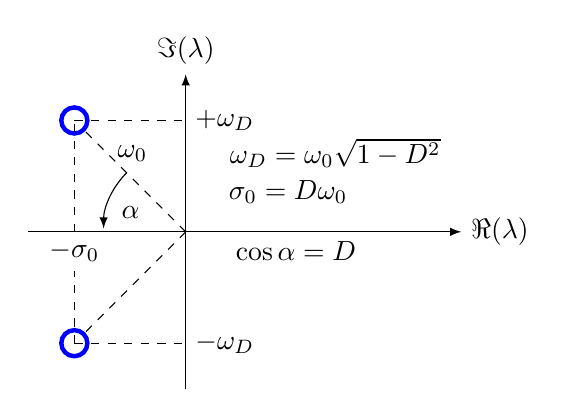
\begin{tikzpicture}
\draw [-latex] (-2,0) -- (3.5,0) node [right]  {$\Re(\lambda)$};
\draw [-latex] (0,-2) -- (0,2) node [above] {$\Im(\lambda)$};
\draw[dashed] (0,0) -- node[pos=0.7, right] {$\omega_0$}(135:2) node[solid, fill=white, circle, draw=blue, ultra thick] {};
\draw[dashed] (0,0) -- node[pos=0.6, above right] {$ $}(-135:2) node[solid, fill=white, circle, draw=blue, ultra thick] {};
\draw[dashed] (-1.4142,0) -- (-1.4142,+1.4142);
\draw[dashed] (-1.4142,-1.4142) -- (-1.4142,-0.5) node [left, above] {$-\sigma_0$};
\draw[dashed] (-1.4142,+1.4142) -- (0,+1.4142) node [right] {$+\omega_D$};
\draw[dashed] (-1.4142,-1.4142) -- (0,-1.4142) node [right] {$-\omega_D$};
\draw[black, -latex] (-0.75,0.75) arc (135:180:1);
\node at (1.9,1) {$\omega_D = \omega_0 \sqrt{1-D^2}$};
\node at (1.3,0.5) {$\sigma_0 = D \omega_0$};
\node at (-0.7,0.25) {$\alpha$};
\node at (1.4,-0.25) {$\cos \alpha = D$};
\end{tikzpicture}}
\subcaptionbox{\textbf{Poles} in complex $s$-plane of LTI system's transfer function, cf. Sec. \ref{sec:TransferFunction}.}[.4\textwidth]{%
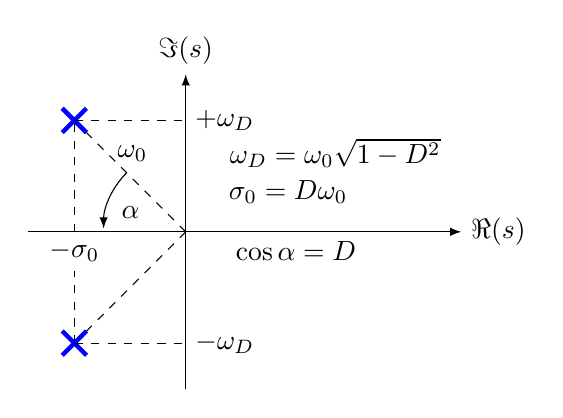
\begin{tikzpicture}
\draw [-latex] (-2,0) -- (3.5,0) node [right]  {$\Re(s)$};
\draw [-latex] (0,-2) -- (0,2) node [above] {$\Im(s)$};
\draw[dashed] (0,0) -- node[pos=0.7, right] {$\omega_0$}(135:2) node[solid, fill=white, cross=6pt, draw=blue, ultra thick] {};
\draw[dashed] (0,0) -- node[pos=0.6, above right] {$ $}(-135:2) node[solid, fill=white, cross=6pt, draw=blue, ultra thick] {};
\draw[dashed] (-1.4142,0) -- (-1.4142,+1.4142);
\draw[dashed] (-1.4142,-1.4142) -- (-1.4142,-0.5) node [left, above] {$-\sigma_0$};
\draw[dashed] (-1.4142,+1.4142) -- (0,+1.4142) node [right] {$+\omega_D$};
\draw[dashed] (-1.4142,-1.4142) -- (0,-1.4142) node [right] {$-\omega_D$};
\draw[black, -latex] (-0.75,0.75) arc (135:180:1);
\node at (1.9,1) {$\omega_D = \omega_0 \sqrt{1-D^2}$};
\node at (1.3,0.5) {$\sigma_0 = D \omega_0$};
\node at (-0.7,0.25) {$\alpha$};
\node at (1.4,-0.25) {$\cos \alpha = D$};
\end{tikzpicture}}
\caption{Sketch of ODE's homogeneous solution case III with a complex conjugate
solution.}
\label{fig:sketch_lambda_plane}
\end{figure}


%##############################################################################
\subsubsection{Specific Parameters}
For our chosen quantities
$\omega_0=\frac{5}{4}$,
$\sigma_0 = \frac{3}{4}$,
$\omega_D=1$
the ODE reads
\begin{align}
\frac{16}{25} \ddot{y} + \frac{24}{25} \dot{y} + y = x.
\end{align}
Some tasks in this exercise require the initial conditions
$\dot{y}(0)=0$ and $y(0)=0$.
Then the Laplace transform becomes
\begin{align}
\boxed{
Y(s) = \frac{X(s)}{\frac{16}{25} s^2 + \frac{24}{25} s + 1}}\,.
\end{align}
Other tasks require initial conditions $\dot{y}(0)=2$ and $y(0)=1$.
Then the Laplace transform reads
\begin{align}
\boxed{
Y(s) = \frac{X(s)}{\frac{16}{25} s^2 + \frac{24}{25} s + 1}+
\frac{\frac{16}{25} s + \frac{56}{25}}{\frac{16}{25} s^2 + \frac{24}{25} s + 1}}\,.
\end{align}

We require the following input signals for this exercise
\begin{itemize}
  \item $x(t) = \delta(t) \quad \laplace \quad X(s) = 1$
  \quad ROC: $s \in \mathbb{C}$
  \item $x(t) = \epsilon(t) \quad \laplace \quad X(s) = \frac{1}{s}$
  \quad ROC: $\Re(s)>0$
  \item $x(t) =  \sin(\omega_D t) \epsilon(t) \quad \laplace \quad
   X(s) = \frac{\omega_D}{s^2 + \omega_D^2}$
   \quad ROC: $\Re(s)>0$ with $\omega_D=1$
\end{itemize}


%##############################################################################
%##############################################################################
\subsection{Solutions Using Laplace Transform}

%##############################################################################
\subsubsection{Task a) with Laplace Transform / Impulse Response}
\label{sec:TransferFunction}
We shall find the inverse Laplace transform
$y(t) = \mathcal{L}^{-1}\{Y(s)\}$ for
\begin{align}
Y(s) = \frac{1}{\frac{16}{25} s^2 + \frac{24}{25} s + 1}
\quad \text{ROC}: \Re(s) > -\frac{3}{4}.
\end{align}
Since the \textbf{Dirac Delta impulse} is the \textbf{input signal} here,
$Y(s)$ is here and only here by definition equivalent with the
\textbf{transfer function} $H(s)$, for which the \textbf{fundamental theorem}
\begin{align}
\boxed{y(t) = x(t)*h(t) \quad \laplace \quad Y(s) = X(s) \cdot H(s)}
\end{align}
connects time and Laplace domain.
%
The inverse Laplace transform can be conveniently solved by carefully
rearranging
$Y(s)$ to
\begin{align}
H(s) = Y(s) = \frac{\frac{25}{16}}{s^2 + \frac{24}{16} s + \frac{25}{16}}=
\frac{25}{16} \cdot \frac{1}{(s + \frac{3}{4})^2 + 1^2}
\end{align}
corresponding to a damped sine function (cf. Appendix) as the LTI system's
impulse response
\begin{align}
\boxed{h(t) = y_\text{Task a}(t) = \frac{25}{16} \e^{-\frac{3}{4} t} \sin(t)
\cdot \epsilon(t)}\,.
\end{align}

Feel free to double check this solution at Wolfram Alpha with input
\begin{verbatim}
InverseLaplaceTransform[1/(16/25*s^2+24/25*s+1)]
\end{verbatim}

We should make ourselves comfortable with the Laplace transform pairs of sine, cosine
functions and its exponentially damped versions in the Appendix.
These will often appear as solutions for ODEs under discussion.


%##############################################################################
\subsubsection{Task b) with Laplace Transform / Step Response}
We shall find the inverse Laplace transform $y(t) = \mathcal{L}^{-1}\{Y(s)\}$
for
\begin{align}
Y(s) = \frac{\frac{1}{s}}{\frac{16}{25} s^2 + \frac{24}{25} s + 1}
\quad \text{ROC}: \Re(s) > 0.
\end{align}
%
We solve this problem by means of partial fraction decomposition.
We have a single pole in the origin $s_{\infty,1}=0$ and a complex conjugate
pole pair $s_{\infty,2,3}=-\frac{3}{4}\pm \im$.
Thus, the Ansatz is
\begin{align}
Y(s) = \frac{1}{s}
\cdot \frac{1}{\frac{16}{25} s^2 + \frac{24}{25} s + 1} =
\frac{A}{s-s_{\infty,1}} + \frac{Bs+C}{(s-s_{\infty,2})(s-s_{\infty,3})}.
\end{align}
Rearranging yields
\begin{align}
1 =
A \cdot (\frac{16}{25} s^2 + \frac{24}{25} s + 1) +
(B s + C) \cdot s.
\end{align}
Comparison of coefficients for $s^2, s^1, s^0$ yields
\begin{align}
  A = 1\quad B = -\frac{16}{25} \quad C = -\frac{24}{25}.
\end{align}
Inserting these into the Ansatz leads to
\begin{align}
Y(s) =
\frac{1}{s} - \left[\frac{\frac{16}{25} s + \frac{24}{25}}{\frac{16}{25} s^2 + \frac{24}{25} s + 1}\right]=
\frac{1}{s} - \left[\frac{s + \frac{3}{2}}{s^2 + \frac{3}{2} s + \frac{25}{16}}\right]=
\frac{1}{s} - \left[\frac{s + \frac{3}{2}}{(s + \frac{3}{4})^2 + 1^2}\right].
\end{align}
Now, the denominator of the second fraction looks well for sine or cosine related
Laplace transforms.
Another rearranging step (this is the part, where some experience
is helpful to bring fractions to a suitable form)
\begin{align}
Y(s) =
\frac{1}{s} - \left[\frac{s + \frac{3}{4}}{(s + \frac{3}{4})^2 + 1^2} +
\frac{\frac{3}{4}}{(s+\frac{3}{4})^2 + 1^2}\right]
\end{align}
splits the term in the bracket.
Individual inverse Laplace transform of each fraction is allowed due to
linearity. Thus, we get
\begin{align}
\boxed{y(t)_\text{Task b} =
\left[1
- \e^{-\frac{3}{4} t} \cos(t)
- \frac{3}{4}\e^{-\frac{3}{4} t} \sin(t) \right] \cdot \epsilon(t)}\,.
\end{align}

Feel free to double check this solution at Wolfram Alpha with input
\begin{verbatim}
InverseLaplaceTransform[(1/s)/(16/25*s^2+24/25*s+1)]
\end{verbatim}

%##############################################################################
\subsubsection{Task c) with Laplace Transform}
We shall find the inverse Laplace transform $y(t) = \mathcal{L}^{-1}\{Y(s)\}$
for
\begin{align}
Y(s) =
\frac{\frac{16}{25} s + \frac{56}{25}}{\frac{16}{25} s^2 + \frac{24}{25} s + 1}
\quad \text{ROC}: \Re(s) > -\frac{3}{4}.
\end{align}
This particular problem becomes solvable by rearranging the fraction to
\begin{align}
Y(s) =
\frac{s + \frac{7}{2}}{s^2 + \frac{3}{2} s + \frac{25}{16}} =
\frac{s + \frac{7}{2}}{(s + \frac{3}{4})^2 + 1^2}
=\frac{s + \frac{3}{4}}{(s + \frac{3}{4})^2 + 1^2}
+\frac{\frac{11}{4}}{(s + \frac{3}{4})^2 + 1^2}.
\end{align}
This results in exponentially damped cosine and sine functions
\begin{align}
\boxed{y(t)_\text{Task c} =
\left[\e^{-\frac{3}{4} t} \cos(t)
+\frac{11}{4}\e^{-\frac{3}{4} t} \sin(t) \right] \cdot \epsilon(t)}\,.
\end{align}

Feel free to double check this solution at Wolfram Alpha with input
\begin{verbatim}
InverseLaplaceTransform[(16/25*s+56/25)/(16/25*s^2+24/25*s+1)]
\end{verbatim}


%##############################################################################
\subsubsection{Task d) with Laplace Transform}
We shall find the inverse Laplace transform $y(t) = \mathcal{L}^{-1}\{Y(s)\}$
for
\begin{align}
Y(s) = \frac{\frac{1}{s}}{\frac{16}{25} s^2 + \frac{24}{25} s + 1}+
\frac{\frac{16}{25} s + \frac{56}{25}}{\frac{16}{25} s^2 + \frac{24}{25} s + 1}
\quad \text{ROC}: \Re(s) > 0.
\end{align}
Straightforward superposition is just to be done here:
We already have calculated the individual inverse Laplace transforms in task b
and c. So the solution becomes
\begin{align}
\boxed{y(t)_\text{Task d} = y(t)_\text{Task b} + y(t)_\text{Task c}
= \left[1+\mathrm{e}^{-\frac{3}{4} t} \, 2 \sin(t) \right] \cdot \epsilon(t)
}\,.
\end{align}
We have observed this characteristics in the time domain as well.

Feel free to double check this solution at Wolfram Alpha with input
\begin{verbatim}
InverseLaplaceTransform[(1/s+16/25*s+56/25)/(16/25*s^2+24/25*s+1)]
\end{verbatim}


%##############################################################################
\subsubsection{Task e) with Laplace Transform}
We shall find the inverse Laplace transform $y(t) = \mathcal{L}^{-1}\{Y(s)\}$
for
\begin{align}
Y(s) = \frac{\frac{1}{s^2 + 1^2}}{\frac{16}{25} s^2 + \frac{24}{25} s + 1}
\quad \text{ROC}: \Re(s) > 0.
\end{align}
Here we deal with two complex conjugate pole pairs (the first one from system
characteristic, the second from the $sin(t)$-input signal)
\begin{align}
s_{\infty,1,2} = -\frac{3}{4} \pm \im \qquad s_{\infty,3,4} = \pm \im.
\end{align}
We again try to solve with partial fraction decomposition, here with the Ansatz
\begin{align}
Y(s) = \frac{A s + B}{\frac{16}{25} s^2 + \frac{24}{25} s + 1}+
\frac{C s + D}{s^2+1}.
\end{align}
Hence,
\begin{align}
1=
(A s + B) \cdot (s^2+1)+
(C s + D) \cdot (\frac{16}{25} s^2 + \frac{24}{25} s + 1).
\end{align}
Manual comparison of coefficients becomes more and more inconvenient with growing
numbers of coefficients.
Although, in this example a matrix inversion is more calculus effort than plain
comparison of coefficients, we should keep in mind that we can set up a system
of linear equations in matrix notation
%wolfram alpha:
%inv[[[0, 1, 0, 1], [10/13, 10/13, 1, 1], [250/137, 125/137, 274/137, 1], [750/241, 250/241, 723/241, 1]]]*[1, 5/13, 25/137, 25/241]
% \begin{align}
% \underbrace{
% \begin{pmatrix}
% 0 & 1 & 0 & 1\\
% \nicefrac{10}{13} & \nicefrac{10}{13} & 1 & 1\\
% \nicefrac{250}{137} & \nicefrac{125}{137} & \nicefrac{274}{137} & 1\\
% \nicefrac{750}{241} & \nicefrac{250}{241} & \nicefrac{723}{241} & 1
% \end{pmatrix}
% }_{\mathbf{M}}
% \cdot
% \underbrace{
% \begin{pmatrix}
% A \\
% B\\
% C\\
% D
% \end{pmatrix}
% }_{\mathbf{u}}
% =
% \underbrace{
% \begin{pmatrix}
% 1\\
% \nicefrac{5}{13}\\
% \nicefrac{25}{137}\\
% \nicefrac{25}{241}
% \end{pmatrix}
% }_{\mathbf{v}}
% \end{align}
% when inserting $s=0,1,2,3$ (included in the ROC) to obtain four equations.
%
%
%
%inv[[[1, 0, 16/25, 0], [0, 1, 24/25, 16/25], [1, 0, 1, 24/25], [0, 1, 0, 1]]]*[0, 0, 0, 1]
\begin{align}
\underbrace{
\begin{pmatrix}
1 & 0 & \nicefrac{16}{25} & 0\\
0 & 1 & \nicefrac{24}{25} & \nicefrac{16}{25}\\
1 & 0 & 1 & \nicefrac{24}{25}\\
0 & 1 & 0 & 1
\end{pmatrix}
}_{\mathbf{M}}
\cdot
\underbrace{
\begin{pmatrix}
A \\
B\\
C\\
D
\end{pmatrix}
}_{\mathbf{u}}
=
\underbrace{
\begin{pmatrix}
0\\
0\\
0\\
1
\end{pmatrix}
}_{\mathbf{v}}
.
\end{align}
%
The matrix $\mathbf{M}$ is full rank (if we do not believe this, we should assure
us. However, it is worth to note that the system response is unique, thus the defined
linear system of equations must be also unique,
requiring that square $\mathbf{M}$ is invertible, which in fact it is).
%
Thus, solving $\mathbf{u} = \mathbf{M}^{-1} \cdot \mathbf{v}$ (in later practice
we might leave this job for a computer, such as e.g. input to Wolfram Alpha
\begin{verbatim}
inv[[[1, 0, 16/25, 0], [0, 1, 24/25, 16/25], [1, 0, 1, 24/25], [0, 1, 0, 1]]]*[0, 0, 0, 1]
\end{verbatim}
) yields the coefficients
\begin{align}
\label{eq:coeffABCDsinLaplace}
  A = \frac{128}{219}
  \quad B = \frac{48}{73}
  \quad C = -\frac{200}{219}
  \quad D = \frac{25}{73}.
\end{align}
%
%
Inserting these into the Ansatz results in
\begin{align}
Y(s) = \frac{\frac{128}{219} s +
\frac{48}{73}}{\frac{16}{25} s^2 +
\frac{24}{25} s + 1} +
\frac{-\frac{200}{219} s +
\frac{25}{73}}{s^2+1}.
\end{align}
This again needs to be reformulated such that \textbf{Laplace transforms of
exponentially damped and undamped sine/cosine functions}
can be revealed (this is a typical exam task).
%
The last fraction is straightforward with regard to that:
\begin{align}
Y(s) = \frac{\frac{128}{219} s + \frac{48}{73}}{\frac{16}{25} s^2 + \frac{24}{25} s + 1}
-\frac{200}{219}\frac{s}{s^2+1^2}
+\frac{25}{73}\frac{1}{s^2+1^2}.
\end{align}
%
The first fraction is similar to the approaches of tasks a) - d) and can be
rearranged as
\begin{align}
Y(s) = &
\frac{\frac{200}{219} s + \frac{75}{73}}{s^2 + \frac{3}{2} s + \frac{25}{16}}
-\frac{200}{219}\frac{s}{s^2+1^2}
+\frac{25}{73}\frac{1}{s^2+1^2}\\
&
\frac{\frac{200}{219} s + \frac{75}{73}}{(s + \frac{3}{4})^2 + 1^2}
-\frac{200}{219}\frac{s}{s^2+1^2}
+\frac{25}{73}\frac{1}{s^2+1^2}\\
&
\frac{200}{219} \frac{s + \frac{3}{4}}{(s + \frac{3}{4})^2 + 1^2}+
\frac{\frac{25}{73}}{(s + \frac{3}{4})^2 + 1^2}
-\frac{200}{219}\frac{s}{s^2+1^2}
+\frac{25}{73}\frac{1}{s^2+1^2}.
\end{align}
This term now can be conveniently transformed back into time domain,
fraction by fraction due to the linearity of the Laplace transform
\begin{align}
\boxed{
  y_\text{Task e}(t) =
  \left[ \frac{200}{219} \e^{-\frac{3}{4} t} \cos(t) +
  \frac{25}{73} \e^{-\frac{3}{4} t} \sin(t) -
  \frac{200}{219} \cos(t) +
  \frac{25}{73} \sin(t) \right] \cdot \epsilon(t)}\,.
\end{align}

Feel free to double check this solution at Wolfram Alpha with input
\begin{verbatim}
InverseLaplaceTransform[(1/(s^2+1^2))/(16/25*s^2+24/25*s+1)]
\end{verbatim}



%##############################################################################
\subsubsection{Transfer Function and Frequency Response of the System}
%
With \eq{eq:steadystate_timedomain}
\begin{align}
y(t\gg 2\pi, t\to\infty) = \frac{25}{3 \sqrt{73}}\cdot
\sin\left(t-\tan^{-1}
\left[\frac{\nicefrac{200}{219}}{\nicefrac{25}{73}}\right]\right),
\end{align}
we explored the \textbf{steady state} of the system giving
amplitude and phase offset for $\omega=1$.
%
A convenient way to calculate the steady state for many (all) $\omega$, is to evaluate
the \textbf{Laplace transform}, i.e. \textbf{the transfer function} of the system,
see taks a)
\begin{align}
H(s) = \frac{1}{\frac{16}{25} s^2 + \frac{24}{25} s + 1}
\end{align}
along the
$\im\omega$-axis of the $s$-domain
\begin{align}
H(\im\omega)
= \frac{1}{\frac{16}{25} s^2 + \frac{24}{25} s + 1}\bigg|_{s=\im\omega}
= \frac{1}{\frac{16}{25} (\im\omega)^2 + \frac{24}{25} \im\omega + 1}
= \frac{1}{ (1 -\frac{16}{25} \omega^2) + \im (\frac{24}{25} \omega)}.
\end{align}
This constitutes the \textbf{Fourier transform} $\mathcal{F}\{h(t)\}$
of the impulse response $h(t)$ and is known as
\textbf{frequency response} $H(\im\omega)$ of the system.
%
Typically, $H(\im\omega)$ is complex-valued (only in rare, special cases
it is real-valued), thus it is meaningful to specify the magnitude and the phase
of the complex number $H(\im\omega)$ at each $\omega$.
%
This is depicted in Fig. \ref{fig:frequency_response_mag_phase}: on top magnitude
$|H(\im\omega)|$ over angular frequency $\omega$, at the bottom plot normalized
phase $\angle H(\im\omega) / \pi$ over $\omega$.
%
%We see in the magnitude plot that, lower frequencies ($\omega<1$) can pass,
%while higher frequencies $\omega>3$ are attenuated.
%
%The system characteristics is therefore called \textbf{low-pass} filter or
%\textbf{high-cut} filter.

If we set up $\omega=1$ in the frequency response
\begin{align}
H(\im(\omega=1))
= \frac{1}{ (1 -\frac{16}{25} (1)^2) + \im (\frac{24}{25} (1))}
= \frac{1}{ \frac{9}{25} + \im \frac{24}{25}}
= \frac{\frac{9}{25} - \im \frac{24}{25}}{ \frac{81}{625} + \frac{576}{625}}
\end{align}
the complex number $H(\im(\omega=1)) = \frac{25}{73} - \im \frac{200}{219}$ results.
%
We are familiar with these numbers as they appeared somehow in task e), cf.
$C$ and $D$ in \eq{eq:coeffABCDsinLaplace}.
%
The resulting magnitude and phase
\begin{equation}
|H(\im(\omega=1))| = \frac{25}{3 \sqrt{73}}
\qquad
\angle H(\im(\omega=1)) = -\tan^{-1}
\left[\frac{\nicefrac{200}{219}}{\nicefrac{25}{73}}\right]
= -\tan^{-1}\left[\frac{8}{3}\right]
\end{equation}
are precisely identical with \eq{eq:steadystate_timedomain},
proving that the shown concepts are consistent.
%
Thus, evaluating the frequency response give us information about the steady
state of a system.
%
\begin{figure}[h!]
\centering
\includegraphics[width=0.75\textwidth]{frequency_response_mag_phase}
\caption{Frequency response for the ODE with Laplace function
$H(s) = \left[ \frac{16}{25} s^2 + \frac{24}{25} s + 1 \right]^{-1}$.}
\label{fig:frequency_response_mag_phase}
\end{figure}



%##############################################################################
%##############################################################################
\clearpage
\subsection*{Appendix A}

%##############################################################################
\subsubsection*{Important Laplace Transform Pairs for Right-Sided Signals}
The Dirac Delta Impulse pair reads
\begin{align}
\boxed{\delta(t) \quad \laplace \quad 1 \quad \text{ROC}: \mathbb{C}}\,.
\end{align}
The Heaviside step function pair reads
\begin{align}
\boxed{\epsilon(t) \quad \laplace \quad \frac{1}{s} \quad \text{ROC}: \Re(s)>0}\,.
\end{align}
With the modulation theorem
\begin{align}
\e^{s_0 t} x(t) \quad \laplace \quad X(s-s_0) \quad \{s \, | \, s-\Re(s_0) \in \text{ROC}(X)\}.
\end{align}
we get (this notation conveniently indicates a pole at $s_0$)
\begin{align}
\boxed{\e^{s_0 t} \epsilon(t)\quad \laplace \quad \frac{1}{s-s_0} \quad \text{ROC}: \Re(s)>\Re(s_0)}\,,
\end{align}
and with changed sign (this notation conveniently represents right-sided,
damped signals for $\Re(s_0)>0$ due to a pole at $-s_0$)
\begin{align}
\boxed{\e^{-s_0 t} \epsilon(t)\quad \laplace \quad \frac{1}{s+s_0} \quad \text{ROC}: \Re(s)>\Re(-s_0)}\,.
\end{align}
%
For the special case of $s_0 = \im \omega_0$, the addition of both versions
yields
\begin{align}
(\e^{+\im \omega_0 t} + \e^{-\im \omega_0 t})  \epsilon(t)\quad &\laplace \quad \frac{1}{s-\im \omega_0} + \frac{1}{s+\im \omega_0} \quad \text{ROC}: \Re(s)>0\\
(\e^{+\im \omega_0 t} + \e^{-\im \omega_0 t})  \epsilon(t)\quad &\laplace \quad \frac{(s+\im \omega_0) + (s-\im \omega_0)}{(s-\im \omega_0)(s+\im \omega_0)}\quad \text{ROC}: \Re(s)>0\\
(\e^{+\im \omega_0 t} + \e^{-\im \omega_0 t})  \epsilon(t)\quad &\laplace \quad \frac{2 s}{s^2 + \omega_0^2}\quad \text{ROC}: \Re(s)>0
\end{align}
\begin{align}
\boxed{\cos(\omega_0 t) \epsilon(t)\quad \laplace \quad \frac{s}{s^2 + \omega_0^2}\quad \text{ROC}: \Re(s)>0}\,,
\end{align}
for which the last is due to the Euler identity $\cos(\omega_0 t) = \frac{1}{2} (\e^{+\im \omega_0 t}+\e^{-\im \omega_0 t})$.
%
For $\sin(\omega_0 t) = \frac{1}{2 \im} (\e^{+\im \omega_0 t}-\e^{-\im \omega_0 t})$ a similar
procedure yields
\begin{align}
\boxed{
\sin(\omega_0 t)\epsilon(t)\quad \laplace \quad \frac{\omega_0}{s^2 + \omega_0^2} \quad \text{ROC}: \Re(s)>0}\,.
\end{align}
%
Modulation theorem leads to (note that $s_0 \in \mathbb{C}$, we often encounter $s_0 > 0, \in \mathbb{R}$ in ODEs)
\begin{align}
\boxed{\e^{-s_0 t} \cos(\omega_0) \epsilon(t)\quad \laplace \quad \frac{(s+s_0)}{(s+s_0)^2 + \omega_0^2}\quad \text{ROC}: \Re(s)>\Re(-s_0)}\,,
\end{align}
and
\begin{align}
\boxed{\e^{-s_0 t} \sin(\omega_0) \epsilon(t)\quad \laplace \quad \frac{\omega_0}{(s+s_0)^2 + \omega_0^2}\quad \text{ROC}: \Re(s)>\Re(-s_0)}\,.
\end{align}



%##############################################################################
%##############################################################################
\newpage
\subsection*{Appendix B}
TBD the big picture ODE 1st/2nd, cf. \cite[p.117]{Strang2014}

\bibliography{literatur}
\end{document}
